\documentclass{article}

\usepackage{tikz, tikz-3dplot}


\begin{document}
	\begin{center}
		\tdplotsetmaincoords{70}{115}
		\begin{tikzpicture}[tdplot_main_coords]
			\coordinate (O) at (0,0,0);
			\coordinate (A) at (2,2,4);
			\coordinate (B) at (0,2,4);
			\coordinate (C) at (0,4,4);
			\coordinate (D) at (2,4,4);
			\coordinate (E) at (2,4,2);
			\coordinate (F) at (2,2,2);
			\coordinate (G) at (0,2,2);
			\coordinate (H) at (0,4,2);
			
			\draw [ultra thick] (A) -- (B) -- (C) -- (H) -- (E) -- (F) -- cycle;
			\draw[ultra thick] (A) -- (D) -- (E);
			\draw[ultra thick] (C) -- (D);
			\draw[ultra thick, densely dashed] (F) -- (G) -- (H);
			\draw[ultra thick, densely dashed] (G) -- (B);
			
			\draw[ultra thick, densely dotted] (G) -- (0,2,0);
			\draw[ultra thick, densely dotted] (H) -- (0,4,0);
			\draw[ultra thick, densely dotted] (G) -- (0,0,2);
			\draw[ultra thick, densely dotted] (B) -- (0,0,4);
			
			\draw (A) node[left]{\(A\)};
			\draw (O) node[below]{\(O\)};
			\draw (B) node[above]{\(B\)};
			\draw (C) node[above]{\(C\)};
			\draw (D) node[above]{\(D\)};
			\draw (E) node[below]{\(E\)};
			\draw (F) node[left]{\(F\)};
			\draw (G) node[above right]{\(G\)};
			\draw (H) node[below right]{\(H\)};
			
			\draw[thick,->,>=latex] (0,0,0) -- (4,0,0) node[anchor=north east]{$x$};
			\draw[thick,->,>=latex] (0,0,0) -- (0,6,0) node[anchor=north west]{$y$};
			\draw[thick,->,>=latex] (0,0,0) -- (0,0,6) node[anchor=south]{$z$};
		\end{tikzpicture}

		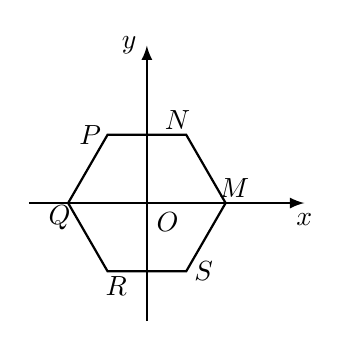
\begin{tikzpicture}
			
			\draw[thick] (0:1) \foreach \j/\l in {1/N,2/P,3/Q,4/R,5/S,6/M} {-- (60*\j:1) node[pos=1.22]{\(\l\)}};
			\draw (0,0) node[below right]{\(O\)};
			\draw[thick, ->, >=latex](-1.5,0) -- (2,0) node[below]{\(x\)};
			\draw[thick, ->, >=latex](0,-1.5) -- (0,2) node[left]{\(y\)};
		\end{tikzpicture}

		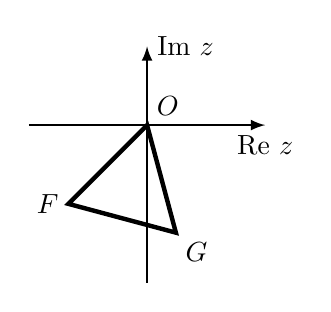
\begin{tikzpicture}
			\coordinate (O) at (0,0);
			\coordinate (F) at (-1,-1);
			\coordinate[rotate around={-60:(F)}] (G);

			\draw[ultra thick] (O) -- (F) -- (G) -- cycle;

			\draw (O) node[above right]{\(O\)};
			\draw (F) node[left]{\(F\)};
			\draw (G) node[below right]{\(G\)};

			\draw[thick, ->, >=latex](-1.5,0) -- (1.5,0) node[below]{Re \(z\)};
			\draw[thick, ->, >=latex](0,-2) -- (0,1) node[right]{Im \(z\)};
		\end{tikzpicture}

		
	\end{center}

	
\end{document}